\documentclass[tikz,multi={tikzpicture},convert={outfile=images/ping-pong.png,density=1000}]{standalone}
\usepackage[build={latexoptions={-output-directory=latex/png}}]{standalone}
\usetikzlibrary{automata, positioning, arrows}
\usepackage{xcolor}
\newcommand{\StIdle}{\tiny\texttt{StIdle}}
\newcommand{\StBusy}{\tiny\texttt{StBusy}}
\newcommand{\StDone}{\tiny\texttt{StDone}}
\newcommand{\MsgPing}{\tiny\texttt{MsgPing}}
\newcommand{\MsgPong}{\tiny\texttt{MsgPong}}
\newcommand{\MsgDone}{\tiny\texttt{MsgDone}}
\newcommand{\StIdleX}{\tiny\texttt{StIdle2}}
\newcommand{\StBusyX}{\tiny\texttt{StBusy2}}
\newcommand{\StDoneX}{\tiny\texttt{StDone2}}
\newcommand{\MsgPingX}{\tiny\texttt{MsgPing2}}
\newcommand{\MsgPongX}{\tiny\texttt{MsgPong2}}
\newcommand{\MsgBusy}{\tiny\texttt{MsgBusy}}
\newcommand{\MsgDoneX}{\tiny\texttt{MsgDone2}}
\definecolor{mygreen}{rgb}{0,0.819608f,0.545098}
\definecolor{myblue}{rgb}{0.172549,0.603922,0.984314}
\begin{document}
\tikzset{
    state/.style={
           rectangle,
           draw=black,
           minimum height=1em,
           inner sep=1pt,
           text centered,
           },
}
\tikzstyle{every node}=[font=\tiny]

% PingPong, v1
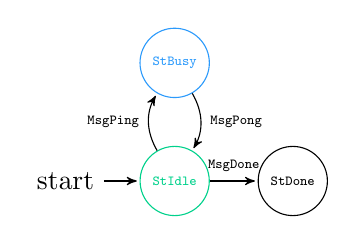
\begin{tikzpicture}[->,>=stealth',shorten >=1pt,auto,node distance=1.5cm]
  \node[state, mygreen, initial]      (Idle) {\StIdle};
  \node[state, right of=Idle]         (Done) {\StDone};
  \node[state, myblue, above of=Idle] (Busy) {\StBusy};

  \draw (Idle) edge[above]             node{\MsgDone} (Done);
  \draw (Idle) edge[left, bend left]  node{\MsgPing} (Busy);
  \draw (Busy) edge[right, bend left] node{\MsgPong} (Idle);
\end{tikzpicture}

% Non-pipelined PingPong client
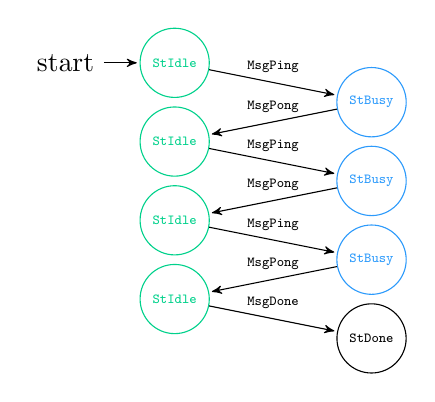
\begin{tikzpicture}[->,>=stealth',shorten >=1pt,auto,node distance=1.5cm]
  \node[state, mygreen, initial] (C0) at (0, 0) {\StIdle};
  \node[state, myblue]           (S0) at (2.5, -0.5) {\StBusy};
  \node[state, mygreen]          (C1) at (0, -1) {\StIdle};
  \node[state, myblue]           (S1) at (2.5, -1.5) {\StBusy};
  \node[state, mygreen]          (C2) at (0, -2) {\StIdle};
  \node[state, myblue]           (S2) at (2.5, -2.5) {\StBusy};
  \node[state, mygreen]          (C3) at (0, -3) {\StIdle};
  \node[state]                   (D)  at (2.5, -3.5) {\StDone};
  \draw (C0) -> node[above]{\MsgPing} (S0);
  \draw (S0) -> node[above]{\MsgPong} (C1);
  \draw (C1) -> node[above]{\MsgPing} (S1);
  \draw (S1) -> node[above]{\MsgPong} (C2);
  \draw (C2) -> node[above]{\MsgPing} (S2);
  \draw (S2) -> node[above]{\MsgPong} (C3);
  \draw (C3) -> node[above]{\MsgDone} (D);
\end{tikzpicture}

% Pipelined PingPong client
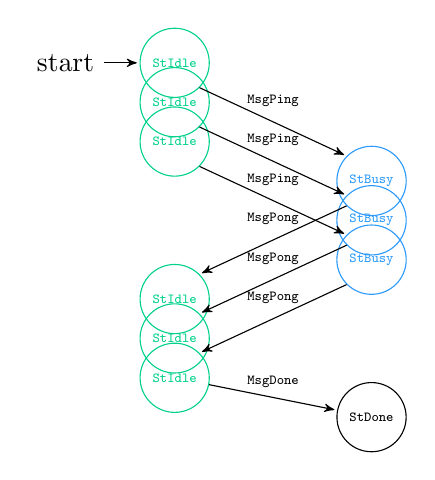
\begin{tikzpicture}[->,>=stealth',shorten >=1pt,auto,node distance=1.5cm]
  \node[state, mygreen, initial] (C0)  at (0, 0)      {\StIdle};
  \node[state, mygreen]          (C1)  at (0, -0.5)   {\StIdle};
  \node[state, mygreen]          (C2)  at (0, -1)     {\StIdle};
  \node[state, myblue]           (S0)  at (2.5, -1.5) {\StBusy};
  \node[state, myblue]           (S1)  at (2.5, -2)   {\StBusy};
  \node[state, myblue]           (S2)  at (2.5, -2.5) {\StBusy};
  \node[state, mygreen]          (C1') at (0, -3)     {\StIdle};
  \node[state, mygreen]          (C2') at (0, -3.5)   {\StIdle};
  \node[state, mygreen]          (C3)  at (0, -4)     {\StIdle};
  \node[state]                   (D)   at (2.5, -4.5) {\StDone};
  \draw[->] (C0.south east) -- node[above=0.07]{\MsgPing} (S0.north west);
  \draw[->] (C1.south east) -- node[above=0.07]{\MsgPing} (S1.north west);
  \draw[->] (C2.south east) -- node[above=0.07]{\MsgPing} (S2.north west);
  \draw[->] (S0.south west) -- node[above=0.07]{\MsgPong} (C1'.north east);
  \draw[->] (S1.south west) -- node[above=0.07]{\MsgPong} (C2'.north east);
  \draw[->] (S2.south west) -- node[above=0.07]{\MsgPong} (C3.north east);
  \draw[->] (C3) -- node[above]{\MsgDone} (D);
\end{tikzpicture}

% PingPong, v2
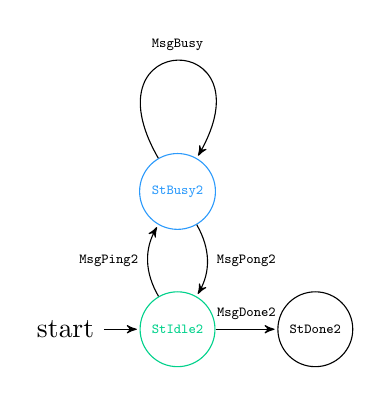
\begin{tikzpicture}[->,>=stealth',shorten >=1pt,auto,node distance=1.75cm]
  \node[state, mygreen, initial]      (Idle) {\StIdleX};
  \node[state, right of=Idle]         (Done) {\StDoneX};
  \node[state, myblue, above of=Idle] (Busy) {\StBusyX};

  \draw (Idle) edge[above]            node{\MsgDoneX} (Done);
  \draw (Idle) edge[left, bend left]  node{\MsgPingX} (Busy);
  \draw (Busy) edge[right, bend left] node{\MsgPongX} (Idle);
  \draw (Busy.120) to [out=120,in=60,looseness=10] node[above]{\MsgBusy} (Busy.60);
\end{tikzpicture}

\end{document}
